% ======================================================================
% Memoria del trabajo grupal — Vulnerabilidades Hardware
% Plantilla TFG ETSI Informática (UMA) con portada propia (portada.tex),
% sin resumen ni contraportada.
% Compilar con: latexmk   (usa XeLaTeX + biber, ver latexmkrc)
% ======================================================================
\documentclass[12pt,a4paper,oneside,spanish]{book}  % spanish: babel y cleveref

%───────── Auxiliary packages ──────────────────────────────────────────
\usepackage[es-noshorthands,es-tabla]{babel}
\usepackage{csquotes}
\usepackage{graphicx}
\usepackage{tikz}   % fondo azul de portada.tex
\usepackage{booktabs}
\usepackage{tabularx}
\usepackage{siunitx}
\usepackage{amsmath,amssymb}
\usepackage{listings}
\usepackage[
  backend=biber,
  style=ieee
]{biblatex}
\addbibresource{referencias.bib}

% Figuras compartidas con la presentación (generadas por los scripts de análisis)
\graphicspath{{../figuras/}}

% Listings config
\lstset{
  basicstyle=\ttfamily\small,
  numbers=left,
  numberstyle=\tiny,
  columns=fullflexible,
  frame=single,
  breaklines=true,
  tabsize=2
}

%───────── Template ────────────────────────────────────────────────────
\usepackage{template/sty_files/template-TFGspanish-uma}

% \cref en español con los mismos nombres que los títulos de la plantilla
\crefname{table}{tabla}{tablas}
\Crefname{table}{Tabla}{Tablas}
\crefname{section}{sección}{secciones}
\Crefname{section}{Sección}{Secciones}

%======================================================================
\begin{document}

% ======================================================================
% Portada de la memoria. Reproduce la portada azul de la plantilla
% (template/sty_files/cotutor_cover-blueuma.sty, v1.4) adaptada a un
% trabajo de asignatura: sin tutor ni departamento y con los cuatro autores.
% Los logos son los de la plantilla, en template/logos/.
% ======================================================================
\begin{titlepage}
  \thispagestyle{empty}%
  \begin{tikzpicture}[remember picture,overlay]
    \fill[UMAblue] (current page.south west) rectangle (current page.north east);
    \node[anchor=north west,xshift=1.5cm,yshift=-1.5cm]
          at (current page.north west)
          {
\includegraphics[width=4.5cm]{template/logos/NEG-uma-logo.png}};
    \node[anchor=north east,xshift=-1.5cm,yshift=-1.5cm]
          at (current page.north east)
          {
\includegraphics[width=9cm]{template/logos/NEG-etsi-logo.png}};
  \end{tikzpicture}%
  \MalacitanaRoman\color{UMAgray}%
  \vspace*{2.5cm}%
  \begin{center}
    {\color{white}\fontsize{16pt}{18pt}\selectfont
      Escuela Técnica Superior de Ingeniería Informática\par}
    \vspace{0.15cm}
    {\fontsize{14pt}{16pt}\selectfont \textit{Vulnerabilidades Hardware}\par}

    \vspace{1.2cm}

    {\color{white}\bfseries\fontsize{20pt}{22pt}\selectfont
      Ataque de análisis de consumo por correlación (CPA) sobre AES-128\par}
    \vspace{0.4cm}
    {\color{white}\fontsize{16pt}{18pt}\selectfont
      Recuperación de la clave en un ATmega328P con un montaje de medida propio\par}

    \vspace{1.2cm}

    {\Large\textit{Realizado por}\par}
    \vspace{0.15cm}
    {\color{white}\Large
      Juan Diego Bermúdez Ureba\par
      Brian Polo Caballero\par
      Alberto Bartolomé Iruela\par
      Roberto Sánchez Martín\par}

    \vfill
    {\Large Universidad de Málaga · Curso 2026/2027\par}
  \end{center}
  \vspace*{0.5cm}%
\end{titlepage}


\frontmatter

%────────────────────── TOC and lists ──────────────────────────────────
\tableofcontents
\clearpage
\listoffigures
\clearpage

\mainmatter
%────────────────────── Capítulo 1 — Introducción ──────────────────────
% Breve resumen con los aspectos más importantes de la vulnerabilidad.
\chapter{Introducción}
\label{cap:introduccion}

\section{Motivación}
% TODO: pregunta de partida: ¿puede filtrarse una clave AES sin leer la
% memoria ni romper el algoritmo? Encuadre dentro de la seguridad hardware
% \cite{mishra2025modern}.

\section{Canales laterales de consumo}
% TODO: qué es un canal lateral, por qué el consumo depende de los datos
% procesados y por qué esto no es un fallo matemático de AES
% \cite{kocher1999dpa,kocher2011intro}.

\section{Objetivos y alcance}
% TODO: demostrar CPA sobre AES-128 software en un ATmega328P propio,
% con clave de laboratorio. Qué queda fuera del alcance.

\section{Estructura del documento}
% TODO: un párrafo que recorra los capítulos siguientes.

%────────────────────── Capítulo 2 — Descripción ───────────────────────
% Detalles sobre el mecanismo de ataque y su implementación.
\chapter{Descripción del ataque}
\label{cap:descripcion}

\section{AES-128 y el valor intermedio atacado}
\label{sec:aes}

AES-128 cifra bloques de 16 bytes con una clave de 16 bytes
\cite{nist2023fips197}. El bloque se copia en un \emph{estado} de 16 bytes, al
que se aplica un primer \texttt{AddRoundKey} con la clave y, después, diez
rondas. Cada ronda encadena cuatro transformaciones: \texttt{SubBytes}, que
sustituye cada byte por su imagen en una tabla fija de 256 entradas (la S-box);
\texttt{ShiftRows}, que rota las filas del estado; \texttt{MixColumns}, que
combina linealmente los bytes de cada columna, y \texttt{AddRoundKey}, que hace
el XOR del estado con una subclave. La última ronda omite \texttt{MixColumns}.
Las once subclaves se obtienen de la clave mediante la expansión de clave. La
S-box es pública y no tiene nada secreto; es el único paso no lineal del
cifrado.

Para el ataque solo importan los dos primeros pasos, que trabajan byte a byte.
El \texttt{AddRoundKey} inicial usa la clave tal cual, así que el byte $j$ del
estado pasa a valer $p_j \oplus k_j$, donde $p_j$ es el byte $j$ del texto
claro y $k_j$ el de la clave. El \texttt{SubBytes} de la primera ronda lo
transforma en
\begin{equation}
  v_j = \mathrm{SBox}(p_j \oplus k_j),
  \label{eq:valor-intermedio}
\end{equation}
que es el valor intermedio que se ataca en este trabajo. Hay dos razones para
elegirlo.

La primera es que depende de un solo byte de clave y de un byte que el atacante
conoce, porque es quien elige el texto claro. Para cada uno de los 256 valores
posibles de $k_j$ se puede calcular qué valor $v_j$ habría procesado el
dispositivo, y comprobar cuál de esas predicciones encaja con el consumo medido.
Cada byte se ataca por separado: en lugar de $2^{128}$ claves hay que
comprobar $16 \times 256 = 4096$ hipótesis.

La segunda explica por qué se ataca la salida de la S-box y no la del XOR, que
también depende solo de $p_j$ y $k_j$. Con el modelo de fuga del peso de
Hamming (\cref{sec:cpa}), la predicción del candidato complementario
$k \oplus \mathtt{0xff}$ sería $\operatorname{HW}(p_j \oplus k \oplus
\mathtt{0xff}) = 8 - \operatorname{HW}(p_j \oplus k)$: exactamente la contraria,
con la misma correlación en valor absoluto que el candidato correcto, y no
habría forma de distinguirlos. Los candidatos que difieren del correcto en un
solo bit también predecirían casi lo mismo. La S-box rompe esa estructura,
porque dos entradas parecidas dan salidas que no se parecen, y solo el candidato
correcto predice bien la fuga.

El mismo razonamiento vale para la última ronda, que no tiene
\texttt{MixColumns}: el byte del criptograma $c_j$ es la salida de la S-box,
desplazada por \texttt{ShiftRows}, combinada por XOR con un byte de la subclave
de la ronda 10. La hipótesis $\mathrm{InvSBox}(c_j \oplus k)$ permite atacar
esa subclave, y como la expansión de clave de AES-128 es invertible, de ella se
deduce la clave. En este trabajo el ataque principal es el de la primera ronda;
el de la última se usa en la simulación como comprobación adicional
(\cref{sec:validacion-simulada}).

\section{Análisis simple de consumo (SPA)}
\label{sec:spa}

El análisis simple consiste en observar una traza, o la media de unas pocas, y
reconocer en ella las operaciones del algoritmo \cite[sec.~II.B.1]{mishra2025modern}.
Cuando el camino de ejecución depende de la clave, como en una exponenciación
modular de RSA que solo multiplica cuando un bit vale uno, el SPA puede revelar
la clave directamente. En el artículo que presentó el DPA ya se distinguían a
simple vista las 16 rondas de un DES en una sola traza \cite{kocher1999dpa}.

Un AES software bien escrito ejecuta las mismas instrucciones sea cual sea la
clave, así que el SPA no basta para atacarlo. En este trabajo sirve para otra
cosa: localizar la primera ronda dentro de la traza, para capturar solo esa
ventana y no buscar a ciegas, y comprobar que el montaje funciona. Que se
distingan las diez rondas en una traza es el primer criterio de validación de la
captura, y todavía no se ha comprobado.
% TODO: traza real con las rondas marcadas cuando el montaje funcione (fase 4).

\section{Análisis diferencial de consumo (DPA)}
\label{sec:dpa}

El DPA de Kocher, Jaffe y Jun \cite{kocher1999dpa} fue el primer ataque
estadístico sobre el consumo. Se miden $N$ cifrados con textos claros aleatorios
y se guarda, para cada uno, la traza $T_i$ y el texto claro $p_i$. Para cada
byte $j$ y cada candidato $k$, una \emph{función de selección} predice un bit
del valor intermedio; aquí, el bit $\ell$ de $\mathrm{SBox}(p_{i,j} \oplus k)$.
Las trazas se reparten en dos grupos, $G_0$ y $G_1$, según el valor predicho de
ese bit, y se restan sus medias en cada instante:
\begin{equation}
  \Delta_j(k, t) = \frac{1}{|G_1|} \sum_{i \in G_1} T_i[t]
                 - \frac{1}{|G_0|} \sum_{i \in G_0} T_i[t].
  \label{eq:dpa}
\end{equation}

Si el candidato es falso, la partición no tiene relación con lo que hace el
dispositivo, los dos grupos son estadísticamente iguales y la diferencia tiende
a cero al crecer $N$. Si es el correcto, en el instante en que se procesa $v_j$
uno de los grupos consume sistemáticamente algo más que el otro y aparece un
pico. El candidato elegido es el que da el pico más alto.

El DPA de un bit desaprovecha información: el dispositivo filtra los ocho bits
de $v_j$ a la vez, y los siete que no se usan para partir se comportan como
ruido. Además, el bit más informativo depende de la implementación y el
atacante no sabe de antemano cuál escoger.

\section{Análisis de consumo por correlación (CPA)}
\label{sec:cpa}

El CPA de Brier, Clavier y Olivier \cite{brier2004cpa} sustituye la partición
por un \emph{modelo de fuga} que predice el consumo entero, y la diferencia de
medias por la correlación de Pearson
\cite[sec.~II.B.3]{mishra2025modern}.

El modelo más habitual es el peso de Hamming $\operatorname{HW}(v)$, el número
de bits a uno del valor procesado, que supone que el consumo en el instante en
que se manipula $v$ es aproximadamente $a \operatorname{HW}(v) + b$ más ruido.
Brier et al.\ proponen en general la distancia de Hamming entre el valor y un
estado de referencia ---el contenido previo del registro o del bus---, del que
el peso de Hamming es el caso con referencia nula. Aquí se usa el peso de
Hamming porque no se conoce qué valor ocupaba antes el registro en el
microcontrolador. Es una hipótesis de trabajo: si las medidas encajan mejor con
otro modelo, se cambiará.

Para cada byte $j$, cada candidato $k$ y cada instante $t$ se calcula la
correlación entre la fuga predicha $h_i = \operatorname{HW}(\mathrm{SBox}(p_{i,j}
\oplus k))$ y la muestra medida $T_i[t]$ sobre las $N$ trazas:
\begin{equation}
  \rho_j(k, t) =
  \frac{\sum_{i=1}^{N} (h_i - \bar h)\,(T_i[t] - \bar T[t])}
       {\sqrt{\sum_{i=1}^{N} (h_i - \bar h)^2}\,\sqrt{\sum_{i=1}^{N} (T_i[t] - \bar T[t])^2}},
  \label{eq:cpa}
\end{equation}
donde $\bar h$ y $\bar T[t]$ son las medias sobre las trazas. El candidato
elegido para el byte $j$ es
\begin{equation}
  \hat k_j = \arg\max_{k} \, \max_{t} \, \lvert \rho_j(k, t) \rvert .
  \label{eq:cpa-decision}
\end{equation}
Se usa el valor absoluto porque el signo de la fuga depende del montaje; por
ejemplo, de en qué lado de la alimentación se coloca el \emph{shunt}.

Con el candidato correcto, la predicción coincide con la fuga real y la
correlación sube en el instante en que se calcula su S-box. Con los otros 255,
la predicción es casi independiente de la traza y la correlación se queda en el
nivel del azar, que baja como $1/\sqrt{N}$. La correlación del candidato
correcto, en cambio, no crece con $N$: depende solo de la relación entre la
varianza de la fuga y la del ruido. La clave aparece cuando el máximo de los
falsos cae por debajo del correcto, y por eso el número de trazas necesario
crece aproximadamente como el inverso del cuadrado de la correlación del
correcto. La \cref{sec:validacion-simulada} cuantifica esta relación sobre
trazas simuladas.

Frente al DPA de un bit, el CPA aprovecha los ocho bits del valor intermedio y
da una medida normalizada, comparable entre bytes y entre montajes. El coste de
cálculo es moderado: $16 \times 256$ correlaciones por instante de la traza,
que se pueden calcular de una vez como un producto de matrices. Además, como la
predicción solo depende del byte de texto claro, basta acumular para cada byte
$j$ y cada uno de los 256 valores de $p_j$ cuántas trazas hay y su suma, sin
guardar las trazas; así lo hace la web explicativa del proyecto.

\section{Implementación experimental}
\label{sec:implementacion}

Esta sección describe el montaje previsto. El análisis ya está implementado y
validado en simulación, pero el instrumental está pendiente de confirmar y el
firmware y la captura todavía no existen. Lo que se dice aquí sobre el
hardware es un diseño, no un resultado: se confirmará o se corregirá con las
medidas del \cref{cap:resultados}.

\subsection{Arquitectura}

El montaje sigue el esquema habitual de los laboratorios de análisis de consumo
sobre firmware, como los de ChipWhisperer \cite{cw-lab-dpa,cw-lab-cpa}, pero con
componentes de propósito general:

\begin{enumerate}
  \item El PC envía por serie un texto claro aleatorio de 16 bytes al
    microcontrolador.
  \item El firmware activa una salida digital de disparo, cifra con la clave de
    laboratorio, desactiva el disparo y devuelve el criptograma.
  \item Un osciloscopio mide en un canal la caída de tensión en una resistencia
    de \emph{shunt} en serie con la alimentación del microcontrolador, que es
    proporcional a su corriente, y en otro la señal de disparo.
  \item El PC comprueba el criptograma con su propia implementación de AES y
    guarda la terna (texto claro, criptograma, traza).
\end{enumerate}

Se repite el proceso miles de veces y las trazas se atacan con el mismo código
que se ha validado en simulación.
% TODO: esquema del montaje en figuras/ cuando esté decidido.

\subsection{Microcontrolador y firmware}

El dispositivo atacado es un ATmega328P, el microcontrolador de 8 bits del
Arduino Nano. Está por decidir si se usa la placa o el chip suelto en una placa
de prototipos. En la placa, el regulador, el conversor USB-serie y los
condensadores de desacoplo comparten alimentación con el microcontrolador, y es
difícil medir solo su corriente; el chip suelto, con su cristal y sus
condensadores, permite colocar el \emph{shunt} solo en su línea de alimentación
o de masa, con el mismo firmware.
% TODO: decisión Nano / chip suelto (AGENTS.md, hardware/README.md).

El firmware implementará un AES-128 software sin protecciones, con
\texttt{SubBytes} como una consulta a tabla byte a byte. Ese recorrido secuencial
del estado es el que hace que cada byte del valor intermedio se procese en su
propia ventana temporal, que es la hipótesis del modelo de trazas simuladas. Se
verificará con los ejemplos del FIPS-197 \cite{nist2023fips197} antes de medir.
% TODO: fase 3. Protocolo serie, velocidad, pin de disparo y commit del
% firmware cuando existan.

\subsection{Medida del consumo}

La corriente del microcontrolador se convierte en tensión con una resistencia
de \emph{shunt} de bajo valor. Si se coloca en la línea de masa, la caída se
puede medir respecto a masa con una sonda normal, aunque hay que vigilar los
bucles de masa entre el PC, la placa y el osciloscopio. Los condensadores de
desacoplo filtran precisamente las variaciones rápidas de corriente que se
quieren medir, así que su posición respecto al \emph{shunt} es una decisión del
diseño.
% TODO: valor del shunt, posición y necesidad de amplificador (preguntas 3 y 4
% de docs/reunion-2026-10-19.md).

El osciloscopio puede ser uno del laboratorio de la universidad o uno USB
comprado; está pendiente de que lo confirme un profesor. Tiene que cumplir tres
requisitos: muestrear lo bastante rápido para resolver la actividad de cada
instrucción, disparar con la señal del firmware o capturarla en un segundo canal
para alinear las trazas después, y poder controlarse desde Python en Linux para
automatizar la campaña. Si el reloj del microcontrolador es demasiado rápido
para el muestreo disponible, se puede reducir, a costa de reajustar la velocidad
del puerto serie.
% TODO: modelo de osciloscopio, frecuencia de muestreo y reloj del MCU, con
% enlace y fecha de consulta de las especificaciones.

\subsection{Procesamiento de las trazas}

El análisis está escrito en Python, con \texttt{numpy} para el cálculo y
\texttt{matplotlib} para las figuras, en el directorio \texttt{analisis/} del
repositorio. Incluye una implementación propia de AES-128, verificada con los
vectores del FIPS-197, de la que salen las predicciones del valor intermedio; el
CPA de la \cref{eq:cpa} y el DPA de la \cref{eq:dpa}, vectorizados sobre los 256
candidatos y todas las muestras; las métricas que se reportan (correlación
frente al tiempo, pico por candidato, puesto de la clave correcta frente al
número de trazas) y el generador de trazas sintéticas de la
\cref{sec:validacion-simulada}. Con una semilla fija, la salida es idéntica
entre ejecuciones, y la integración continua lo comprueba en cada cambio.

Las trazas reales se guardarán en un fichero \texttt{.npz} por campaña con las
trazas, los textos claros, los criptogramas y la clave, más un \texttt{.json}
de metadatos con la frecuencia de muestreo, el reloj del microcontrolador, el
\emph{shunt}, el osciloscopio, la fecha y la versión del firmware. Antes del
ataque habrá que alinear las trazas con la señal de disparo y, si es necesario,
recortarlas a la ventana de la primera ronda que se identifique por SPA.
% TODO: alineación y preprocesado reales cuando haya trazas (fase 4).

%────────────────────── Capítulo 3 — Mitigaciones ──────────────────────
% Enumeración de posibles mitigaciones y su impacto.
\chapter{Mitigaciones}
\label{cap:mitigaciones}

El ataque del \cref{cap:descripcion} necesita dos cosas: que el consumo en un
instante concreto dependa de un valor intermedio que el atacante puede predecir,
y que pueda repetir la medida las veces suficientes para que la estadística
saque esa dependencia del ruido. Las contramedidas atacan una de las dos.
Mangard, Oswald y Popp las agrupan en dos familias \cite{mangard2007power}: el
\emph{ocultamiento} (\emph{hiding}), que reduce la relación señal-ruido haciendo
el consumo constante o impredecible en el tiempo, y el \emph{enmascaramiento}
(\emph{masking}), que hace que los valores que se procesan dejen de ser
predecibles aunque el consumo siga dependiendo de ellos. A estas se suman las
medidas de protocolo, como la renovación de claves, que limitan cuántas trazas
puede reunir el atacante con una misma clave. La revisión de Mishra y Sahay
recoge las tres \cite[secs.~II.C.5 y III.D]{mishra2025modern}.

Ninguna de ellas es una garantía absoluta. Cada una sube el coste del ataque
---más trazas, mejor equipo, un modelo más elaborado---, y casi todas tienen un
coste para el defensor en tiempo de ejecución, área, energía o complejidad.
Las secciones siguientes describen cada una, su coste y sus límites, y qué
efecto tendría sobre el ataque de este trabajo.

\section{Enmascaramiento (\emph{masking})}
\label{sec:masking}

El enmascaramiento combina cada valor sensible con un número aleatorio nuevo en
cada ejecución, la \emph{máscara}, y opera sobre el valor enmascarado. En el
enmascaramiento booleano, en lugar de $v$ se manipula $v \oplus m$, con $m$
uniforme y desconocida para el atacante. Cada valor que pasa por el procesador
es, por separado, independiente de la clave, y la predicción
$\operatorname{HW}(\mathrm{SBox}(p_j \oplus k))$ del CPA deja de correlar con
el consumo de cualquier instante. Chari et al.\ formalizaron la idea dividiendo
cada valor en varias partes aleatorias y demostraron que, si cada parte se mide
con ruido, el número de trazas necesario crece exponencialmente con el número de
partes \cite{chari1999masking}.

En AES, las operaciones lineales (\texttt{AddRoundKey}, \texttt{ShiftRows},
\texttt{MixColumns}) se aplican a cada parte por separado. La S-box no es
lineal y obliga a algo más: en software, lo habitual es calcular en cada
ejecución una tabla enmascarada $\mathrm{SBox}'(x \oplus m) = \mathrm{SBox}(x)
\oplus m'$ \cite{herbst2006aes}. Eso cuesta memoria para la
tabla, tiempo para recalcularla y una fuente de números aleatorios en el
dispositivo.

El límite principal es que el enmascaramiento de primer orden solo protege
frente a ataques que miran un instante. Un atacante que combina las muestras de
dos instantes ---el de la máscara y el del valor enmascarado--- recupera una
dependencia con la clave: es el DPA de segundo orden, que Messerges ya aplicó en
2000 contra software enmascarado \cite{messerges2000second}. Más partes elevan
el orden del ataque necesario, y con ruido suficiente su coste, pero también el
del cifrado. Además, la protección depende de que las partes no se combinen
nunca en el hardware sin querer, por ejemplo al sobrescribir un registro que
contenía una con la otra, y eso es difícil de garantizar en un procesador real.
% TODO: fuente concreta (capítulo de Mangard et al. sobre ataques a
% implementaciones enmascaradas, o artículo específico).

Contra el ataque de este trabajo, una implementación enmascarada correcta haría
fallar el CPA de primer orden tal como está escrito, independientemente del
número de trazas.

\section{Aleatorización y \emph{shuffling}}
\label{sec:shuffling}

La aleatorización no oculta el valor, sino el momento en que se procesa. El CPA
compara las trazas instante a instante, así que supone que la S-box del byte $j$
se calcula siempre en la misma muestra. Hay dos formas de romper esa
alineación en software:

\begin{itemize}
  \item \emph{Shuffling}: procesar los 16 bytes del estado en un orden
    aleatorio distinto en cada cifrado. Las operaciones de AES son las mismas
    en cualquier orden, y el coste es pequeño: generar una permutación por
    cifrado \cite{herbst2006aes}.
  \item Retardos aleatorios: insertar entre las operaciones bucles de duración
    aleatoria, de modo que todo lo que viene detrás se desplaza
    \cite{clavier2000countermeasures}. Cuesta tiempo de ejecución, en
    proporción a la longitud media de los retardos.
\end{itemize}

El efecto sobre el CPA se puede estimar con el razonamiento de la
\cref{sec:cpa}. Si la S-box de un byte cae con la misma probabilidad en
cualquiera de $m$ posiciones, en cada una solo está presente en una de cada $m$
trazas, y su correlación se reduce aproximadamente a $\rho/m$. Como el número
de trazas crece como el inverso del cuadrado de la correlación, harían falta
del orden de $m^2$ veces más. Con el \emph{shuffling} de 16 bytes, $m = 16$. El
atacante puede compensarlo en parte sumando las $m$ ventanas posibles antes de
correlar, como proponen Clavier et al.\ frente a los retardos aleatorios
\cite{clavier2000countermeasures}; si el ruido de las ventanas es independiente,
la correlación queda en torno a $\rho/\sqrt{m}$ y el factor baja a unas $m$
veces. Estas estimaciones salen de un modelo simple y no se han comprobado
sobre trazas: medirlas es el objetivo de la fase opcional de contramedidas.
% TODO: si se hace la fase 6, comparar con las trazas necesarias medidas.

El límite de la aleatorización es que no elimina la fuga, solo la diluye: con
suficientes trazas, el ataque vuelve a funcionar. Por eso se combina con el
enmascaramiento, como en la implementación de Herbst et al.\ para tarjetas
inteligentes de 8 bits \cite{herbst2006aes}. Además, si el SPA permite
reconocer los retardos en una traza individual, se pueden eliminar alineando las
trazas antes del ataque.

\section{Lógica balanceada}
\label{sec:logica-balanceada}

Las lógicas balanceadas atacan la causa física de la fuga. En la lógica de
doble raíl con precarga, cada bit se representa con dos señales
complementarias que se precargan a un valor fijo en cada ciclo y después se
evalúan: en cada ciclo cambia exactamente una de las dos, sea cual sea el
dato, y el consumo es en principio independiente del valor
\cite{tiri2004wddl}. WDDL (\emph{wave dynamic differential logic}) implementa
esa idea con celdas estándar, de modo que se puede aplicar en ASIC o en FPGA
\cite{tiri2004wddl}; Mishra y Sahay la citan entre las contramedidas hardware
frente al DPA \cite[sec.~III.D]{mishra2025modern}.

El coste es alto: se duplican las señales y se añade la fase de precarga, lo que
aumenta el área, el consumo y el tiempo de cada operación. El límite es que el
equilibrio nunca es perfecto, porque las dos líneas de cada par no tienen
exactamente la misma capacidad tras el rutado, y esa diferencia residual
vuelve a depender del dato \cite{mangard2007power}.
% TODO: fuente: precisar el capítulo de Mangard et al. (ocultamiento).

Esta contramedida se decide al diseñar el circuito. En un microcontrolador
comercial como el ATmega328P, que no la incorpora, no se puede aplicar desde el
firmware.

\section{Inyección de ruido}
\label{sec:ruido}

Otra forma de ocultamiento es añadir consumo que no depende de los datos: un
generador de ruido en la alimentación, circuitos que conmutan al azar o, en
software, operaciones falsas intercaladas con las reales
\cite[sec.~III.D]{mishra2025modern}. El objetivo es bajar la relación
señal-ruido de la medida.

Es una de las medidas más baratas, pero su efecto sobre el CPA es limitado
porque el ruido independiente de los datos se cancela al promediar. La
simulación de la \cref{sec:validacion-simulada} lo ilustra: al pasar de una
relación señal-ruido de 0,2 a 0,02, las trazas que necesita el 90~\% de los
ensayos pasan de 295 a 2220, unas 7,5 veces más (\cref{tab:sim-ruido}). El ataque se encarece de forma lineal, no exponencial
como con el enmascaramiento, y un atacante con tiempo y un buen equipo de
captura lo compensa. Por eso el ruido se usa como complemento de otras medidas y
no como protección única.

\section{Renovación de claves (\emph{re-keying})}
\label{sec:rekeying}

La renovación de claves no toca la implementación del cifrado, sino el uso que
se hace de él. Si cada clave cifra menos bloques de los que el atacante
necesita para recuperarla, el CPA no llega a converger. En el esquema de
\emph{fresh re-keying} de Medwed et al., cada sesión cifra con una clave nueva
que se deriva de la clave maestra y de un número aleatorio público; la función
de derivación se elige para que sea fácil de proteger, de modo que solo ella
necesita contramedidas costosas, y el cifrado de cada sesión se puede dejar sin
proteger \cite{medwed2010fresh}. Mishra y Sahay mencionan también la opción de
fijar el intervalo de renovación a partir del número de trazas que necesita un
ataque \cite[sec.~II.C.5]{mishra2025modern}.

Su límite es que desplaza el problema en lugar de eliminarlo: la clave maestra
sigue en el dispositivo y la derivación sigue siendo un objetivo. Además,
requiere cambiar el protocolo, porque las dos partes tienen que sincronizar la
clave de cada sesión, y no protege frente a ataques que necesitan muy pocas
trazas, como los de plantillas \cite[sec.~II.B.4]{mishra2025modern}.

En el modelo simulado, con una relación señal-ruido de 0,1, la mediana de
trazas para recuperar la clave completa está entre 296 y 413
(\cref{tab:sim-ruido}). Una clave que se renovara cada pocas decenas de
cifrados quedaría fuera del alcance de ese ataque, pero el umbral real depende
del montaje y no se conoce hasta medir.

\section{Tiempo constante no es protección frente al consumo}
\label{sec:tiempo-constante}

Una implementación de tiempo constante ejecuta las mismas instrucciones, en el
mismo orden y con la misma duración, sea cual sea la clave. Protege frente a los
ataques de tiempo \cite{kocher1996timing} y frente al SPA basado en el flujo de
ejecución, pero no frente al DPA ni al CPA: el consumo de cada instrucción sigue
dependiendo de los valores que manipula. De hecho, un código de tiempo constante
favorece al atacante de consumo, porque produce trazas perfectamente alineadas.
Es exactamente la situación del modelo simulado de la
\cref{sec:validacion-simulada}, en el que el CPA recupera la clave.

\section{Resumen}
\label{sec:resumen-mitigaciones}

La \cref{tab:mitigaciones} resume las contramedidas. Su coste y su eficacia
se indican de forma cualitativa, porque dependen de la implementación y no se
han medido en este trabajo.

\begin{table}[htbp]
  \centering
  \caption{Resumen de las contramedidas frente al análisis de consumo. Las
    valoraciones son cualitativas y proceden de las referencias citadas en
    cada sección.}
  \label{tab:mitigaciones}
  \small
  \begin{tabularx}{\textwidth}{>{\raggedright\arraybackslash}p{2.9cm}
                               >{\raggedright\arraybackslash}p{1.8cm}
                               >{\raggedright\arraybackslash}X
                               >{\raggedright\arraybackslash}X}
    \toprule
    Contramedida & Nivel & Efecto sobre el CPA & Límite principal \\
    \midrule
    Enmascaramiento & Algoritmo & Anula el CPA de primer orden &
      Ataques de orden superior; combinación accidental de las partes \\
    \emph{Shuffling} y retardos & Algoritmo & Diluye el pico; más trazas &
      No elimina la fuga; integración de ventanas y realineado \\
    Lógica balanceada & Circuito & Reduce la fuga en origen &
      Desequilibrio residual; solo en diseño de hardware \\
    Inyección de ruido & Circuito o software & Baja la SNR; más trazas &
      El ruido se cancela al promediar \\
    Renovación de claves & Protocolo & Limita las trazas por clave &
      La derivación de claves sigue expuesta; cambia el protocolo \\
    \bottomrule
  \end{tabularx}
\end{table}

%────────────────────── Capítulo 4 — Resultados ────────────────────────
% Análisis de los resultados, a ser posible sobre máquinas reales.
% Solo datos medidos o simulados por nosotros; las simulaciones se
% etiquetan como tales. Las figuras salen de los scripts de análisis.
\chapter{Resultados}
\label{cap:resultados}

\section{Validación del análisis con trazas simuladas}
\label{sec:validacion-simulada}
% Todos los números y figuras de esta sección salen de:
%   uv run python -m analisis.run_all
% (analisis/experiments.py, analisis/figures.py y analisis/config.py).
% Los resultados numéricos quedan en analisis/salida/resultados.json, que no
% se sube al repositorio porque se regenera con la misma semilla.

Antes de medir nada conviene comprobar que el ataque está bien implementado y
saber qué cabe esperar de él. Para eso se generan \emph{trazas sintéticas} con
el modelo de fuga de la \cref{sec:cpa} ---peso de Hamming del valor intermedio
más ruido gaussiano--- y se atacan con el mismo código que después se aplicará
a las trazas medidas. \textbf{Todo lo que aparece en esta sección es
simulación}: no son medidas de ningún montaje y no dicen nada sobre el
microcontrolador, que todavía no se ha instrumentado.

\subsection{Modelo de las trazas simuladas}

Cada traza sintética se construye sumando a la fuga buscada cuatro
perturbaciones que también aparecen en una medida real:

\begin{equation}
  T_i[t] = \underbrace{b_i}_{\text{offset}}
         + \underbrace{d_i[t]}_{\text{deriva}}
         + \underbrace{n_i[t]}_{\text{ruido}}
         + \sum_{r} g_r \cdot \operatorname{HW}\!\left(V_i^{(r)}\right) \cdot k[t - t_r],
  \label{eq:modelo-traza}
\end{equation}

donde $V^{(1)}_i = \mathrm{SBox}(p_i \oplus k)$ es la salida de la S-box de la
primera ronda, $V^{(10)}_i = \mathrm{InvSBox}(c_i \oplus k)$ la entrada de la
S-box de la última, $k[\cdot]$ un núcleo $(0{,}5,\,1{,}0,\,0{,}5)$ que reparte
cada operación en tres muestras consecutivas y $t_r$ el instante central de la
operación del byte $r$. La separación entre ventanas es de dos muestras, como
correspondería a un recorrido byte a byte del estado en el microcontrolador.
La relación señal-ruido se define sobre la potencia de la fuga,
$\mathrm{SNR} = \operatorname{Var}\!\left(\sum_r g_r \operatorname{HW}(V^{(r)})\right) / \sigma_n^2$,
que es lo que permite comparar campañas con distinto ruido. El desplazamiento
$b_i$ es constante dentro de una traza: infla la varianza de la traza y por
tanto rebaja algo la correlación medida, pero no cambia el orden de los
candidatos, porque la correlación de Pearson lo elimina.

Los parámetros concretos de la campaña de referencia ---4000 trazas de 96
muestras, $\mathrm{SNR} = 0{,}1$, semilla \num{20261018}--- están en
\texttt{analisis/config.py} y se guardan en el JSON de resultados, de modo que
la ejecución se puede repetir exactamente. La \cref{fig:sim-trazas} muestra
cómo son.

\begin{figure}[htbp]
  \centering
  % Generada por analisis/figures.py::figure_synthetic_traces
  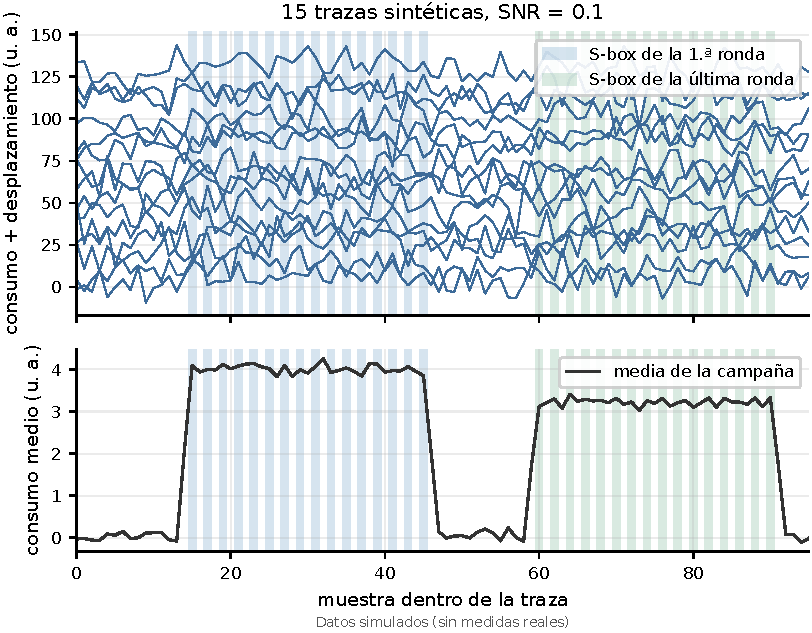
\includegraphics[width=\textwidth]{sim-trazas.pdf}
  \caption{Trazas sintéticas de la campaña de referencia (arriba, quince
    trazas superpuestas con un desplazamiento vertical para distinguirlas) y
    su media (abajo). Las bandas señalan la ventana temporal de la S-box de la
    primera ronda (azul) y de la última (verde). En la media se ve el escalón
    del peso de Hamming de cada byte del estado. \textbf{Datos simulados.}}
  \label{fig:sim-trazas}
\end{figure}

\subsection{Comprobación del AES}

El valor intermedio que ataca el CPA tiene que ser exactamente el de la norma,
o el ataque buscaría una clave distinta de la real. La implementación de
referencia se comprueba contra los vectores de ejemplo del FIPS-197
\cite{nist2023fips197}: el ejemplo del apéndice~B, el caso trivial del apéndice
C.1 y dos casos con clave o texto claro todo a uno. En los cuatro se verifica
el cifrado y el descifrado, y además se comprueba que la versión vectorizada
---la que genera las trazas--- produce byte a byte el mismo resultado que la
versión directa. Estas comprobaciones forman parte de
\texttt{uv run python -m analisis.tests} y se ejecutan antes de generar
cualquier figura.

\subsection{Recuperación de la clave}

La \cref{fig:sim-cpa-correlacion} muestra el resultado central del ataque sobre
la campaña de referencia. Arriba está el coeficiente de correlación del
candidato correcto de cada uno de los 16 bytes; abajo, el mayor de los 255
candidatos falsos. La diferencia es nítida: el candidato correcto llega a
$|\rho| \approx \num{0,22}$ justo en la ventana de su byte, mientras que
ningún candidato falso pasa de $\num{0,07}$. Los 16 bytes de la clave se
recuperan con 4000 trazas, tanto atacando la primera ronda
($\overline{|\rho|} = \num{0,221}$, mínimo $\num{0,212}$) como la última
($\overline{|\rho|} = \num{0,184}$). La cota teórica para esta campaña es
$\rho_{\max} = \sqrt{\mathrm{SNR}/(1+\mathrm{SNR})} = \num{0,302}$; la
diferencia se explica por el desplazamiento por traza de la
\cref{eq:modelo-traza}, que engorda la varianza de la traza y baja la cota a
$\num{0,286}$ en estas condiciones.

\begin{figure}[htbp]
  \centering
  % Generada por analisis/figures.py::figure_correlation_over_time
  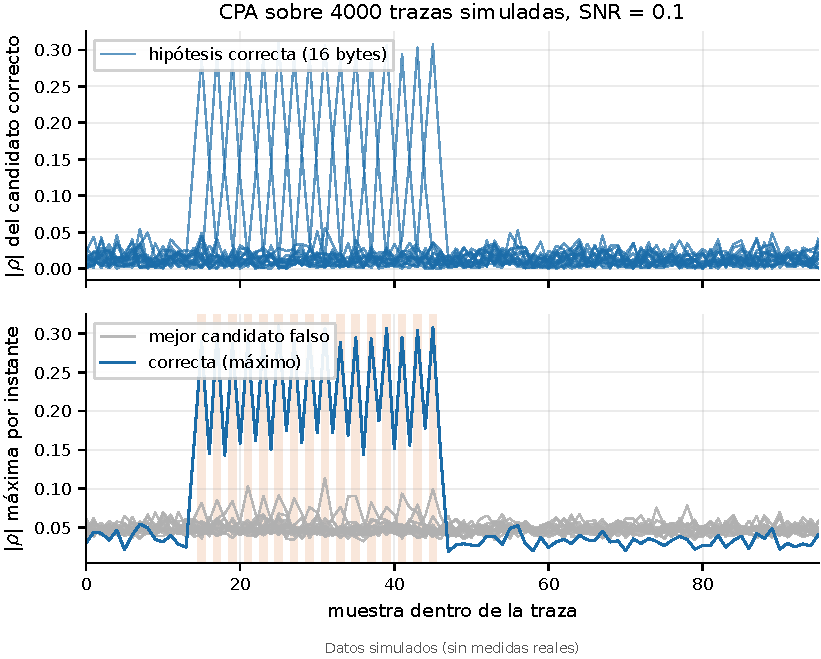
\includegraphics[width=\textwidth]{sim-cpa-correlacion.pdf}
  \caption{Correlación de Pearson frente al tiempo, sobre 4000 trazas
    simuladas con $\mathrm{SNR} = 0{,}1$. Arriba, el candidato correcto de
    cada uno de los 16 bytes; abajo, el mejor candidato falso de cada byte,
    que se queda muy por debajo. Las bandas marcan las ventanas de la S-box.
    \textbf{Datos simulados.}}
  \label{fig:sim-cpa-correlacion}
\end{figure}

La \cref{fig:sim-candidatos} ordena los 256 candidatos por su pico de
correlación y muestra en qué puesto queda el correcto. La separación entre el
primero y el resto es el margen del ataque: $\overline{\Delta|\rho|} =
\num{0,146}$ en la primera ronda, y el candidato correcto es el primero en los
16 bytes. El ataque acierta también en el \emph{tiempo}: el pico del byte $j$
cae en la muestra $15 + 2j$, que es donde el simulador colocó su operación.

\begin{figure}[htbp]
  \centering
  % Generada por analisis/figures.py::figure_peaks_per_candidate
  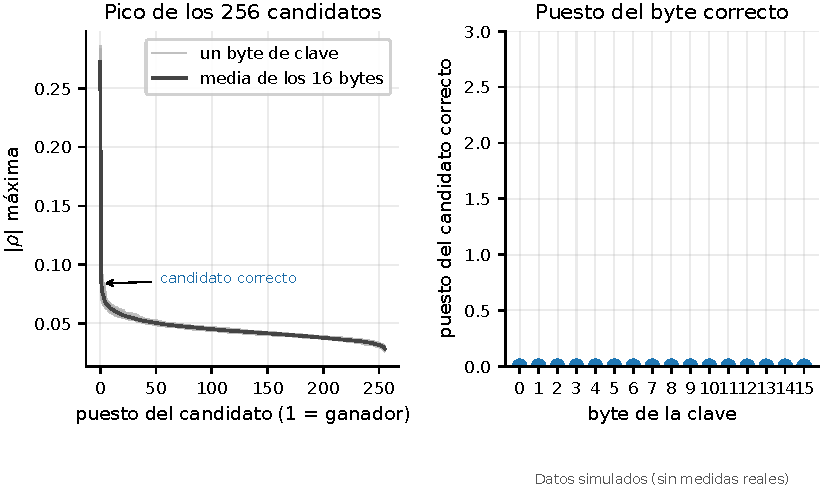
\includegraphics[width=\textwidth]{sim-candidatos.pdf}
  \caption{Izquierda: pico de $|\rho|$ de los 256 candidatos de cada byte,
    ordenados de mayor a menor, más la media de los 16 bytes. Derecha: puesto
    que ocupa la hipótesis correcta en cada byte (1 = ganador).
    \textbf{Datos simulados.}}
  \label{fig:sim-candidatos}
\end{figure}

\subsection{Cuántas trazas y cuánto ruido}

El número de trazas y el ruido son los dos factores que deciden si el ataque
funciona. Para medirlo se repite el CPA completo sobre 60 campañas
independientes de 3000 trazas ---con clave y textos claros nuevos en cada
una--- en nueve niveles de ruido, y se anota en qué puesto queda el byte
correcto de cada posición. El resultado está en la
\cref{fig:sim-rango} para la campaña de referencia y en la
\cref{tab:sim-ruido} para todos los niveles.

\begin{figure}[htbp]
  \centering
  % Generada por analisis/figures.py::figure_rank_curve y figure_noise_scaling
  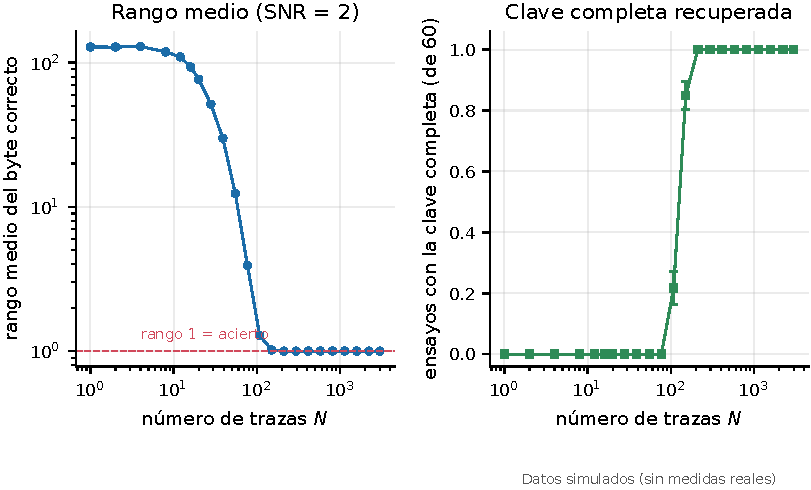
\includegraphics[width=\textwidth]{sim-rango.pdf}
  \caption{Izquierda: rango medio del byte correcto frente al número de trazas
    ($\mathrm{SNR} = 0{,}1$, media de 60 ensayos). Derecha: proporción de
    ensayos en los que se recuperan los 256 bits. \textbf{Datos simulados.}}
  \label{fig:sim-rango}
\end{figure}

\begin{table}[htbp]
  \centering
  \caption{Trazas necesarias para recuperar los 256 bits en función del ruido.
    «N para el 90~\%» es el primer número de trazas en el que la media de los
    60 ensayos lo consigue; «N mediana», la mediana del primer instante en que
    lo consigue cada ensayo. La última columna es el pico medio de $|\rho|$ del
    candidato correcto con 3000 trazas. \textbf{Datos simulados.}}
  \label{tab:sim-ruido}
  \begin{tabular}{S[table-format=1.3] S[table-format=4.0] S[table-format=4.0] S[table-format=1.3]}
    \toprule
    {SNR} & {N para el 90~\%} & {N mediana} & {pico de $|\rho|$} \\
    \midrule
    2      & 211  & 151  & 0,515 \\
    1      & 211  & 211  & 0,466 \\
    0,5    & 295  & 295  & 0,400 \\
    0,2    & 578  & 413  & 0,300 \\
    0,1    & 1133 & 809  & 0,227 \\
    0,05   & 1586 & 1586 & 0,166 \\
    0,02   & \multicolumn{1}{c}{$>$3000} & \multicolumn{1}{c}{$>$3000} & 0,108 \\
    0,01   & \multicolumn{1}{c}{$>$3000} & \multicolumn{1}{c}{$>$3000} & 0,079 \\
    0,005  & \multicolumn{1}{c}{$>$3000} & \multicolumn{1}{c}{$>$3000} & 0,062 \\
    \bottomrule
  \end{tabular}
\end{table}

\begin{figure}[htbp]
  \centering
  % Generada por analisis/figures.py::figure_noise_scaling
  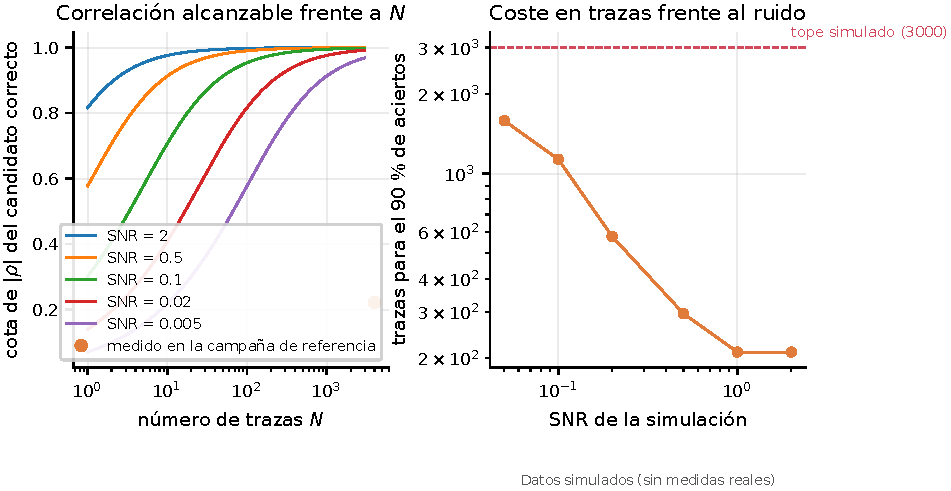
\includegraphics[width=\textwidth]{sim-ruido.pdf}
  \caption{Izquierda: cota teórica de $|\rho|$ en función del número de trazas
    para varios niveles de ruido, con el valor medido en la campaña de
    referencia. Derecha: trazas necesarias para recuperar los 256 bits en el
    90~\% de los ensayos. \textbf{Datos simulados.}}
  \label{fig:sim-ruido}
\end{figure}

Los resultados siguen la ley esperada: la correlación crece como
$\sqrt{N\,\mathrm{SNR}/(1 + N\,\mathrm{SNR})}$, de modo que hacer el ataque
viable con diez veces menos trazas exige diez veces menos ruido. Por debajo de
$\mathrm{SNR} = 0{,}02$ la campaña de 3000 trazas ya no basta y el candidato
correcto se queda fuera del primer puesto en más de la mitad de los ensayos.
Hay que insistir en que estos números son propiedad del \emph{modelo}, no del
montaje: fijan el orden de magnitud que habrá que comparar con las medidas
reales, y solo entonces se podrá decir si el montaje se parece a la simulación.

\subsection{Comparación con el DPA}

El DPA clásico separa las trazas según un único bit del valor intermedio
\cite{kocher1999dpa}, así que aprovecha mucha menos información que el modelo
de peso de Hamming del CPA \cite{brier2004cpa}. La \cref{fig:sim-dpa-cpa} lo
cuantifica sobre la misma campaña de 2000 trazas con $\mathrm{SNR} = 0{,}1$: el
CPA recupera los 16 bytes, mientras que el mejor de los ocho bits del DPA
recupera 8 y el peor, uno solo. La comparación justifica atacar con el peso de
Hamming completo (o con un modelo de fuga más rico) en cuanto el ruido aprieta.

\begin{figure}[htbp]
  \centering
  % Generada por analisis/figures.py::figure_dpa_vs_cpa
  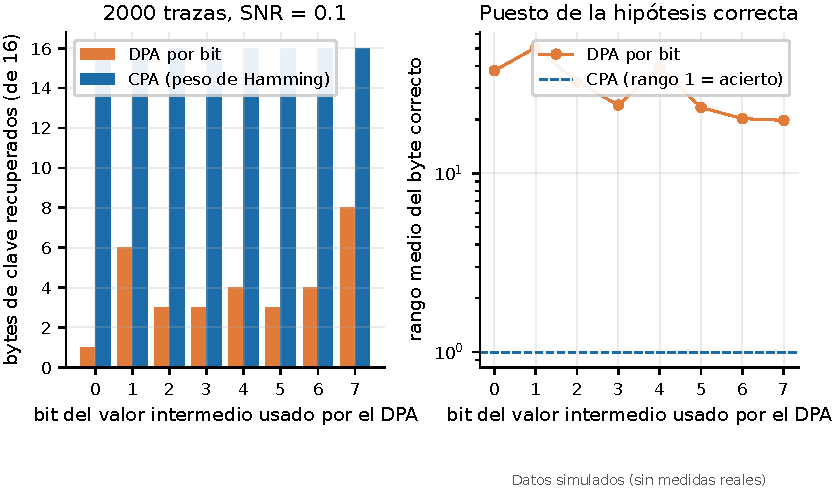
\includegraphics[width=\textwidth]{sim-dpa-cpa.pdf}
  \caption{Izquierda: bytes de clave recuperados por el DPA de cada bit y por
    el CPA sobre la misma campaña de 2000 trazas simuladas
    ($\mathrm{SNR} = 0{,}1$). Derecha: puesto medio de la hipótesis correcta.
    \textbf{Datos simulados.}}
  \label{fig:sim-dpa-cpa}
\end{figure}

\section{Calidad de la captura}
% TODO: traza real, alineación con el trigger, ruido, frecuencia de
% muestreo efectiva frente al reloj del microcontrolador.

\section{Recuperación de la clave}
% TODO: correlación frente al tiempo, correlación máxima por candidato,
% rango de la clave correcta frente al número de trazas y comparación de
% la clave recuperada con la de laboratorio. (Con trazas reales, fase 5.)

\section{Limitaciones}
% TODO: qué condiciones del montaje favorecen o dificultan el ataque.

%────────────────────── Capítulo 5 — Conclusiones ──────────────────────
% Resumen con los puntos fuertes y débiles de la vulnerabilidad.
\chapter{Conclusiones}
\label{cap:conclusiones}

\section{Puntos fuertes del ataque}

\section{Puntos débiles y requisitos}

\section{Trabajo futuro}


%────────────────────── Appendices ─────────────────────────────────────
\begin{umaappendices}
%────────────────────── Anexos ─────────────────────────────────────────
% Información adicional y bibliografía recomendada.
\umaappendix{Detalles del montaje y del código}
% TODO: lista de material, esquema eléctrico, protocolo serie, fragmentos
% relevantes del firmware y de los scripts de análisis.

\umaappendix{Bibliografía recomendada}
% TODO: lecturas comentadas para profundizar \cite{mangard2007power}
% y tutoriales de ChipWhisperer \cite{cw-lab-dpa,cw-lab-cpa}.

\end{umaappendices}

%────────────────────── Bibliography ───────────────────────────────────
\backmatter
\printbibliography[title={Bibliografía}]

\end{document}
% ======================================================================
